%LaTeX reported generated by EES
\documentclass[10pt,fleqn]{article}
\mathindent 0.0in
\usepackage[ansinew]{inputenc}
\usepackage{times}
\usepackage{graphicx}
\usepackage{color}
\definecolor{silver}{rgb}{0.75,0.75,0.75}
\definecolor{gray}{rgb}{0.5,0.5,0.5}
\definecolor{aqua}{rgb}{0.5,1,1}
\definecolor{navy}{rgb}{0.0,0.0,0.5}
\definecolor{orange}{rgb}{1.0,0.5,0.0}
\definecolor{teal}{rgb}{0.25,0.5,0.5}
\definecolor{olive}{rgb}{0.5,0.5,0.0}
\definecolor{purple}{rgb}{0.5,0.0,0.5}
\definecolor{brown}{rgb}{0.5,0.25,0.0}
\definecolor{fuchsia}{rgb}{1.0,0.5,1.0}
\definecolor{buff}{rgb}{1.0,0.94,0.80}
\definecolor{lime}{rgb}{0.5,1.0,0.0}
\setlength{\headsep}{-0.6in}
\setlength{\textheight}{9in}
\setlength{\footskip}{1.0 in}
\setlength{\oddsidemargin}{-0.2in}
\setlength{\evensidemargin}{-0.2in}
\setlength{\textwidth}{6.8in}
\usepackage{longtable}
\newcommand{\abs}[1]{\left|#1\right|}
\newcommand{\F}[1]{\mbox{$#1$}}
\newcommand{\K}[1]{\mbox{\sf#1\ \ \mit}}
\newcommand{\KS}[1]{\mbox{\sf\ \ #1\ \ \mit}}
\newcommand{\SC}[1]{\mbox{`#1'}\  }
\newcommand{\V}[1]{\mbox{$ #1 $}}
\newcommand{\I}{\mbox{\hspace{0.20in}}}
\newcommand{\temperature}{\mathrm{T}}
\newcommand{\pressure}{\mathrm{P}}
\newcommand{\volume}{\mathrm{v}}
\newcommand{\density}{\mathrm{\rho}}
\newcommand{\intenergy}{\mathrm{u}}
\newcommand{\enthalpy}{\mathrm{h}}
\newcommand{\entropy}{\mathrm{s}}
\newcommand{\molarmass}{\mathrm{MW}}
\newcommand{\enthalpyfusion}{\mathrm{\Delta h_{fusion}}}
\newcommand{\quality}{\mathrm{x}}
\newcommand{\viscosity}{\mathrm{\mu}}
\newcommand{\conductivity}{\mathrm{k}}
\newcommand{\prandtl}{\mathrm{P_r}}
\newcommand{\cp}{\mathrm{c_p}}
\newcommand{\cv}{\mathrm{c_v}}
\newcommand{\specheat}{\mathrm{c_p}}
\newcommand{\soundspeed}{\mathrm{c}}
\newcommand{\wetbulb}{\mathrm{wb}}
\newcommand{\humrat}{\mathrm{\omega}}
\newcommand{\acentricfactor}{\mathrm{\omega}}
\newcommand{\relhum}{\mathrm{\phi}}
\newcommand{\dewpoint}{\mathrm{DP}}
\newcommand{\volexpcoef}{\mathrm{\beta}}
\newcommand{\compressibilityfactor}{\mathrm{Z}}
\newcommand{\surfacetension}{\mathrm{\gamma}}
\newcommand{\tcrit}{\mathrm{T_{crit}}}
\newcommand{\pcrit}{\mathrm{P_{crit}}}
\newcommand{\vcrit}{\mathrm{v_{crit}}}
\newcommand{\ttriple}{\mathrm{T_{triple}}}
\newcommand{\fugacity}{\mathrm{fugacity}}
\newcommand{\tsat}{\mathrm{T_{sat}}}
\newcommand{\psat}{\mathrm{P_{sat}}}
\newcommand{\eklj}{\mathrm{ek_{LJ}}}
\newcommand{\sigmalj}{\mathrm{\sigma_{LJ}}}
\newcommand{\isentropicexponent}{\mathrm{k_{s}}}
\newcommand{\thermaldiffusivity}{\mathrm{\alpha}}
\newcommand{\kinematicviscosity}{\mathrm{\nu}}
\newcommand{\isothermalcompress}{\mathrm{K_{T}}}
\begin{document}
\begin{center}
\bf \mbox{MEGN361$\_$EES$\_$MINIPROJECT$\_$JAYD}
\vspace{0.2 in}
\end{center}
\subsection*{Equations}
\begin{verbatim}
$ifnot parametricTable
\end{verbatim}  \begin{equation}
\label{EES Eqn:1}
\V{Pr}  = 11 
\mbox{\I compressor pressure ratio. compression ratio is the same for both gas-turbine and steam-turbine cycles. this is P2/P1}
\end{equation}
\begin{verbatim}
$endif
\end{verbatim}  \begin{equation}
\label{EES Eqn:2}
r_{c} = 11 
\end{equation}
\begin{equation}
\label{EES Eqn:3}
\dot {Q}_{H} = 40\cdot \rm { \left|1000\ \frac {\rm{kW}}{\rm{MW}}\right|} 
\mbox{\I heater input rate}
\end{equation}
\begin{equation}
\label{EES Eqn:4}
\eta_{c,gas} = 0.8 
\mbox{\I isentropic gas compressor efficiency}
\end{equation}
\begin{equation}
\label{EES Eqn:5}
\eta_{t,gas} = 0.85 
\mbox{\I isentropic gas turbine efficiency}
\end{equation}
\begin{equation}
\label{EES Eqn:6}
\eta_{t,steam} = 0.83 
\mbox{\I isentropic steam turbine efficiency}
\end{equation}
\begin{equation}
\label{EES Eqn:7}
\eta_{p,steam} = 0.78 
\mbox{\I isentropic steam pump efficiency}
\end{equation}
\begin{equation}
\label{EES Eqn:8}
e_{he} = 0.70 
\mbox{\I heat exchanger effectiveness}
\end{equation}
\begin{equation}
\label{EES Eqn:9}
\V{T1}  = 25   \   \left[ \rm C \right] 
\mbox{\I temperature at compressor inlet}
\end{equation}
\begin{equation}
\label{EES Eqn:10}
\V{P1}  = 100   \   \left[ \rm kPa \right] 
\mbox{\I pressure at compressor inlet}
\end{equation}
\begin{equation}
\label{EES Eqn:11}
\V{v1}  =\volume \left(\F{Air},\mbox{\ T}=\V{T1} ,\mbox{\ P}=\V{P1}  \right)  
\end{equation}
\begin{equation}
\label{EES Eqn:12}
\V{h1} =\enthalpy \left(\F{Air},\mbox{\ T}=\V{T1}  \right)  
\end{equation}
\begin{equation}
\label{EES Eqn:13}
\V{s1} =\entropy \left(\F{Air},\mbox{\ T}=\V{T1} ,\mbox{\ P}=\V{P1}  \right)  
\end{equation}
\begin{equation}
\label{EES Eqn:14}
\V{P2}  = \V{Pr} \cdot \V{P1}  
\end{equation}
\begin{equation}
\label{EES Eqn:15}
\V{s2}  = \V{s1}  
\mbox{\I isentropic compressor}
\end{equation}
\begin{equation}
\label{EES Eqn:16}
\V{T2} =\temperature \left(\F{Air},\mbox{\ s}=\V{s2} ,\mbox{\ P}=\V{P2}  \right)  
\end{equation}
\begin{equation}
\label{EES Eqn:17}
\V{h2} =\enthalpy \left(\F{Air},\mbox{\ T}=\V{T2}  \right)  
\end{equation}
\begin{equation}
\label{EES Eqn:18}
\V{T3}  = 1300   \   \left[ \rm C \right] 
\mbox{\I turbine inlet temperature}
\end{equation}
\begin{equation}
\label{EES Eqn:19}
\V{P3}  = \V{P2}  
\mbox{\I Constant pressure heat addition}
\end{equation}
\begin{equation}
\label{EES Eqn:20}
\V{h3} =\enthalpy \left(\F{Air},\mbox{\ T}=\V{T3}  \right)  
\end{equation}
\begin{equation}
\label{EES Eqn:21}
\V{s3} =\entropy \left(\F{Air},\mbox{\ T}=\V{T3} ,\mbox{\ P}=\V{P3}  \right)  
\end{equation}
\begin{equation}
\label{EES Eqn:22}
\V{P4}  = \V{P3} \cdot  \left( 1/\V{Pr} \right)  
\end{equation}
\begin{equation}
\label{EES Eqn:23}
\V{s4}  = \V{s3}  
\end{equation}
\begin{equation}
\label{EES Eqn:24}
\V{T4}  = \temperature \left(\F{Air},\mbox{\ s}=\V{s4} ,\mbox{\ P}=\V{P4}  \right)  
\end{equation}
\begin{equation}
\label{EES Eqn:25}
\V{h4}  = \enthalpy \left(\F{Air},\mbox{\ T}=\V{T4}  \right)  
\end{equation}
\begin{equation}
\label{EES Eqn:26}
\V{P5}  = \V{P4}  
\end{equation}
\begin{equation}
\label{EES Eqn:27}
\V{T5}  = \V{T4}  
\end{equation}
\begin{equation}
\label{EES Eqn:28}
\V{h5} =\enthalpy \left(\F{Air},\mbox{\ T}=\V{T5}  \right)  
\end{equation}
\begin{equation}
\label{EES Eqn:29}
\V{P7}  = \V{P6}  
\end{equation}
\begin{equation}
\label{EES Eqn:30}
\V{T7}  = \V{T4}  
\end{equation}
\begin{equation}
\label{EES Eqn:31}
\V{h7} =\enthalpy \left(\F{Steam}_{IAPWS},\mbox{\ T}=\V{T7} ,\mbox{\ P}=\V{P7}  \right)  
\end{equation}
\begin{equation}
\label{EES Eqn:32}
\V{s8} =\entropy \left(\F{Steam}_{IAPWS},\mbox{\ T}=\V{T7} ,\mbox{\ P}=\V{P7}  \right)  
\end{equation}
\begin{equation}
\label{EES Eqn:33}
\V{P8}  = \V{P7} \cdot  \left( 1/r_{c} \right)  
\end{equation}
\begin{equation}
\label{EES Eqn:34}
\V{s8}  = \V{s7}  
\end{equation}
\begin{equation}
\label{EES Eqn:35}
\V{T8} =\temperature \left(\F{Steam}_{IAPWS},\mbox{\ P}=\V{P8} ,\mbox{\ s}=\V{s8}  \right)  
\end{equation}
\begin{equation}
\label{EES Eqn:36}
\V{h8}  = \enthalpy \left(\F{Steam}_{IAPWS},\mbox{\ T}=\V{T8} ,\mbox{\ P}=\V{P8}  \right)  
\end{equation}
\begin{equation}
\label{EES Eqn:37}
\V{P9}  = 100   \   \left[ \rm kPa \right] 
\mbox{\I given}
\end{equation}
\begin{equation}
\label{EES Eqn:38}
\V{T9}  = 99.63   \   \left[ \rm C \right] 
\mbox{\I from table since we know sat liquid}
\end{equation}
\begin{equation}
\label{EES Eqn:39}
\V{h9}  =\enthalpy \left(\F{Steam}_{IAPWS},\mbox{\ T}=\V{T9} ,\mbox{\ P}=\V{P9}  \right)  
\end{equation}
\begin{equation}
\label{EES Eqn:40}
\V{s9} =\entropy \left(\F{Steam}_{IAPWS},\mbox{\ T}=\V{T9} ,\mbox{\ P}=\V{P9}  \right)  
\end{equation}
\begin{equation}
\label{EES Eqn:41}
\V{P6}  = 17\cdot \rm { \left|1000\ \frac {\rm{kPa}}{\rm{MPa}}\right|} 
\end{equation}
\begin{equation}
\label{EES Eqn:42}
\V{s6}  = \V{s9}  
\end{equation}
\begin{equation}
\label{EES Eqn:43}
\V{T6} =\temperature \left(\F{Steam}_{IAPWS},\mbox{\ P}=\V{P6} ,\mbox{\ s}=\V{s6}  \right)  
\end{equation}
\begin{equation}
\label{EES Eqn:44}
\V{h6} =\enthalpy \left(\F{Steam}_{IAPWS},\mbox{\ T}=\V{T6} ,\mbox{\ P}=\V{P6}  \right)  
\end{equation}
\begin{equation}
\label{EES Eqn:45}
\dot {m}_{air} = \frac {\dot {Q}_{H}}{ h3-h2 } 
\end{equation}
\begin{equation}
\label{EES Eqn:46}
\dot {m}_{water} = \dot {m}_{air}\cdot  \left( \frac {\V{h4} -\V{h5} }{ h7-h6 } \right)  
\end{equation}
\begin{equation}
\label{EES Eqn:47}
w_{c} = \V{h2}  - \V{h1}  
\end{equation}
\begin{equation}
\label{EES Eqn:48}
w_{t,gas} = \V{h3} -\V{h4}  
\end{equation}
\begin{equation}
\label{EES Eqn:49}
w_{p} = \V{h6} -\V{h9}  
\end{equation}
\begin{equation}
\label{EES Eqn:50}
w_{t,steam} = \V{h7} -\V{h8}  
\end{equation}
\begin{equation}
\label{EES Eqn:51}
\dot {qsmall}_{h} = \dot {Q}_{H}/\dot {m}_{air} 
\end{equation}
\begin{equation}
\label{EES Eqn:52}
\dot {W}_{brayton} =  \dot {m}_{air}\cdot  \left( w_{t,gas} - w_{c} \right)  
\end{equation}
\begin{equation}
\label{EES Eqn:53}
\dot {W}_{rankine} = \dot {m}_{water}\cdot  \left( w_{t,steam} - w_{p} \right)  
\end{equation}
\begin{equation}
\label{EES Eqn:54}
\dot {W}_{net} = \dot {m}_{air}\cdot  \left( w_{t,gas} - w_{c} \right)  + \dot {m}_{water}\cdot  \left( w_{t,steam} - w_{p} \right)  
\end{equation}
\begin{equation}
\label{EES Eqn:55}
\eta_{brayton} = \dot {W}_{brayton}/\dot {Q}_{H} 
\end{equation}
\begin{equation}
\label{EES Eqn:56}
\eta_{th} = \dot {W}_{net}/\dot {Q}_{H} 
\end{equation}

\vspace{0.10in}
\noindent
\rm As the pressure ratio (Pr) increases, the efficency of the cycle increases as well. The output of the gas turbine results in a lower temperature as efficiency increases

\vspace{0.10in}
\noindent
\rm The performance of the plan can be improved by further inreasing the pressure ratio of the devices in the Brayton cycle.

\subsection*{Plot Window 1:\;Plot\;1}
{\centerline{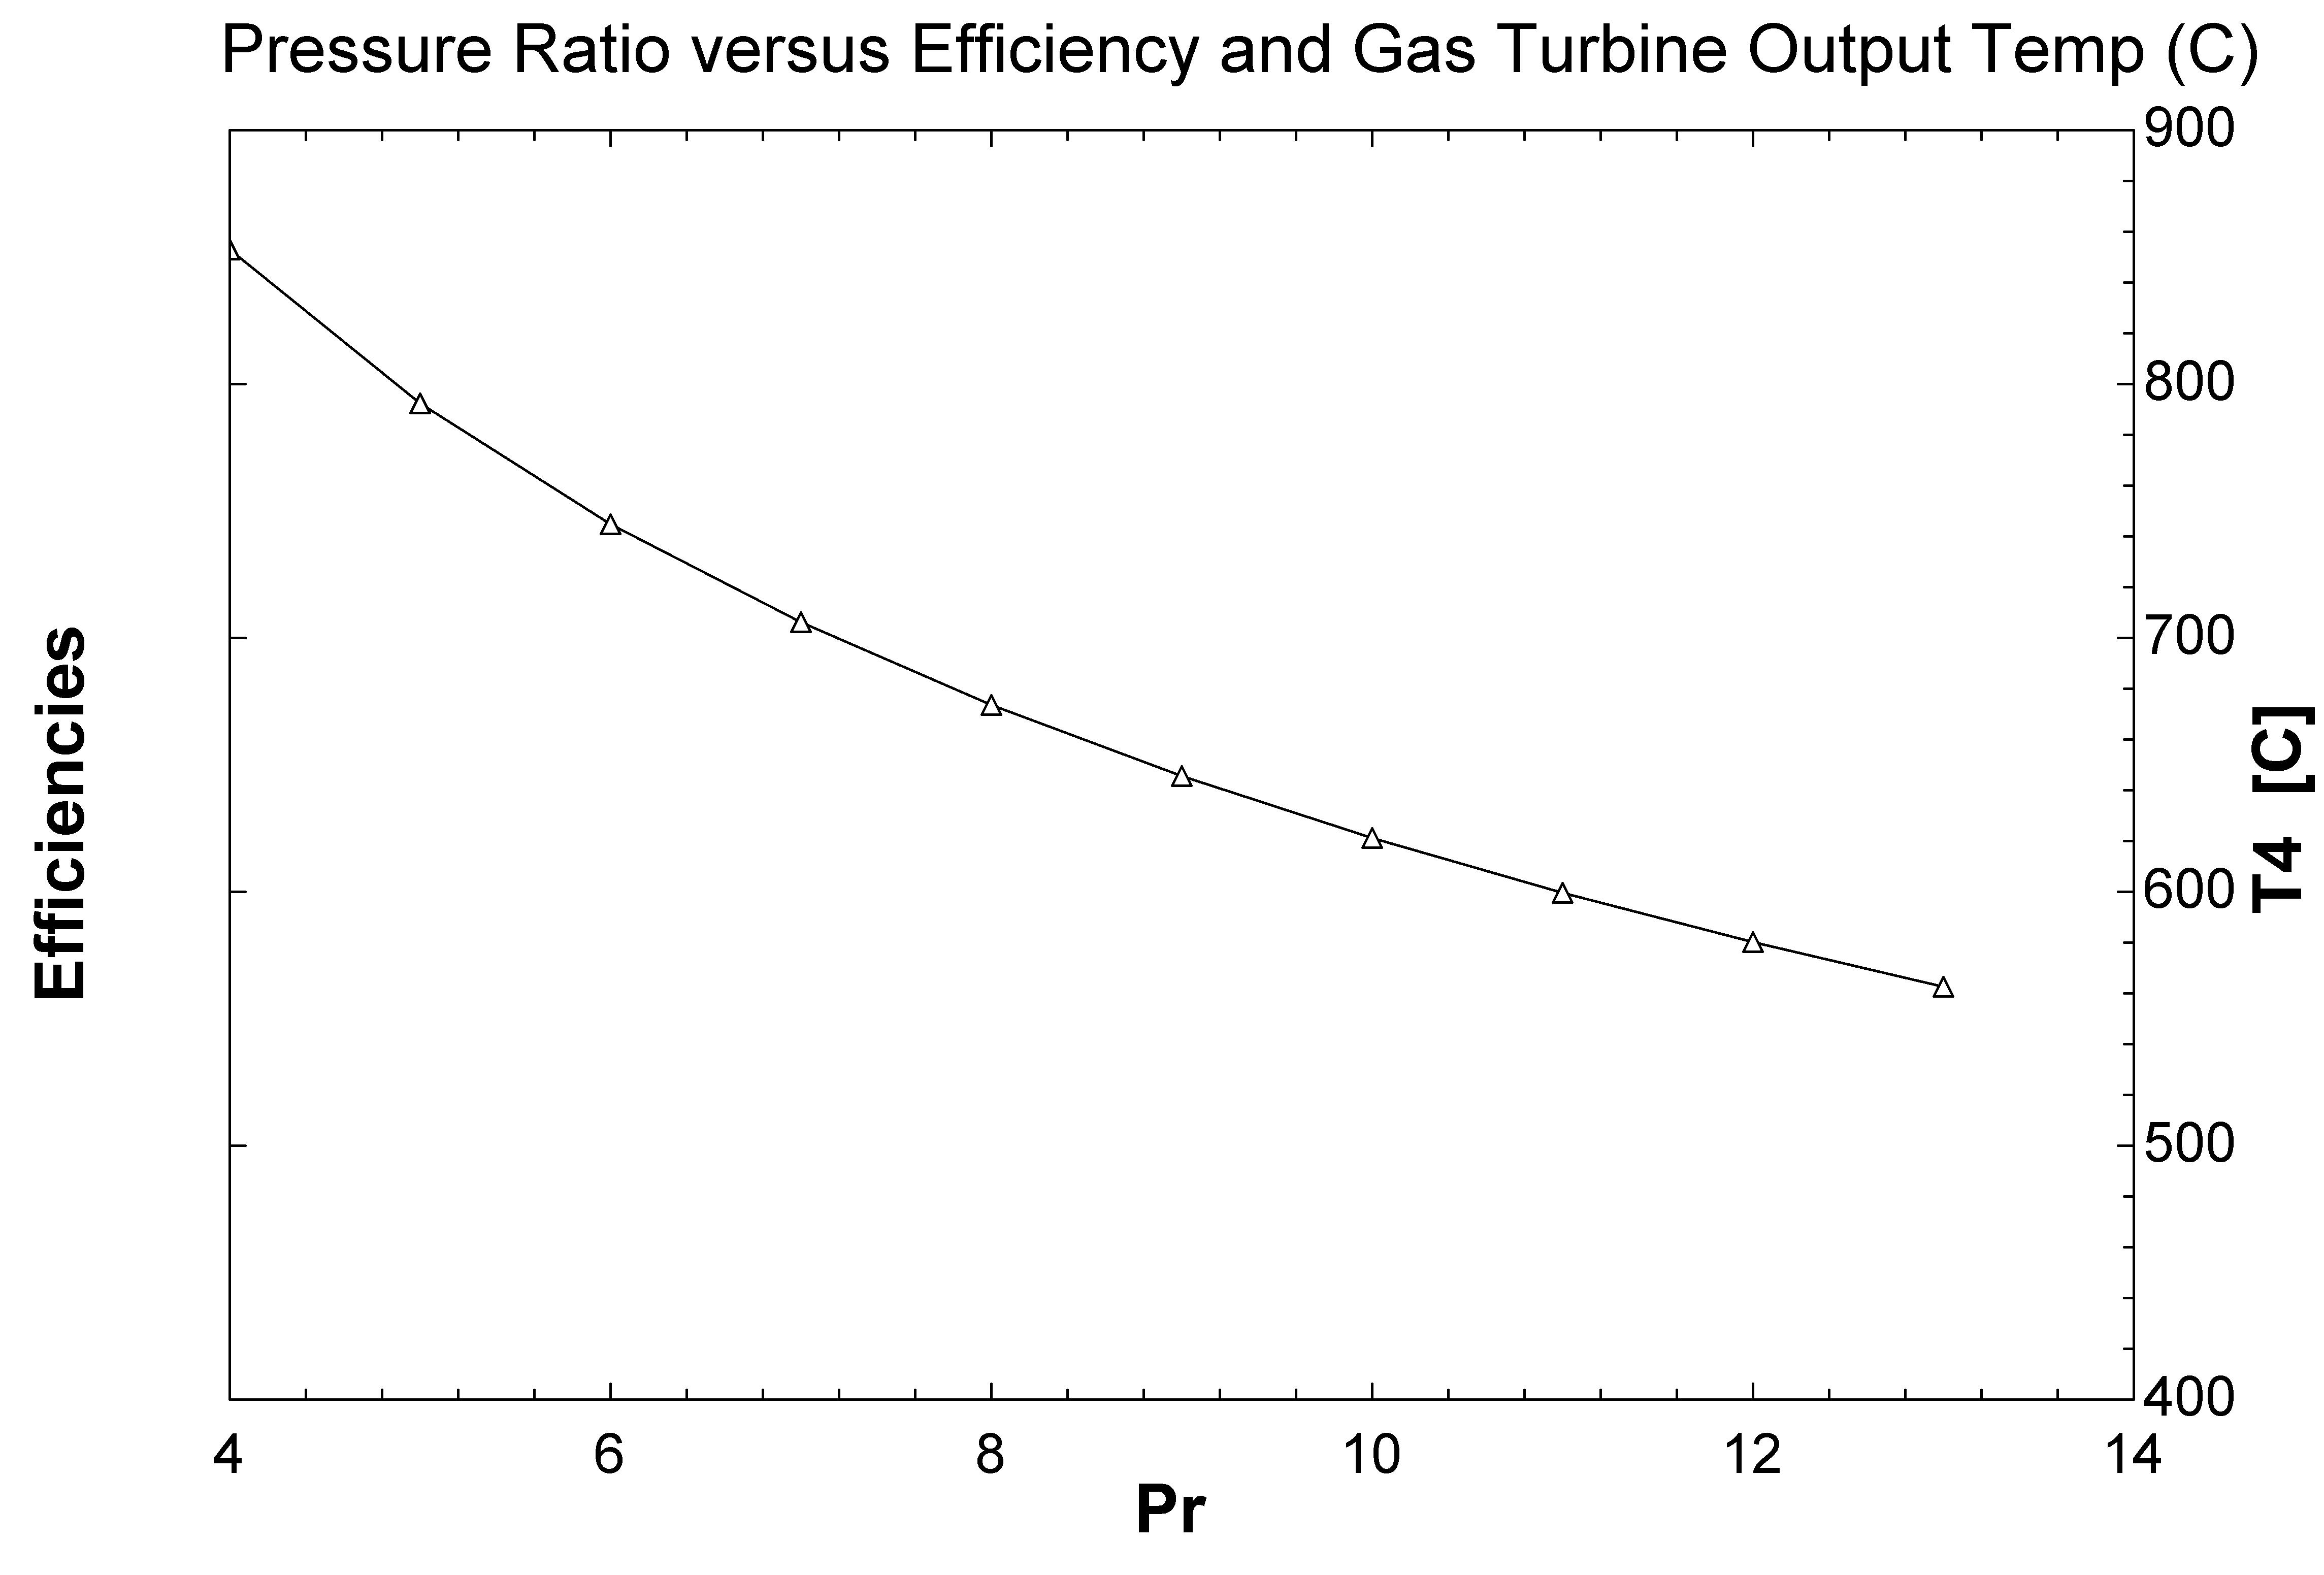
\includegraphics[width=5.0in,keepaspectratio]{megn361_ees_miniProject_JayD_P1.jpg}}
\subsection*{Plot Window 3:\;Plot\;3}
{\centerline{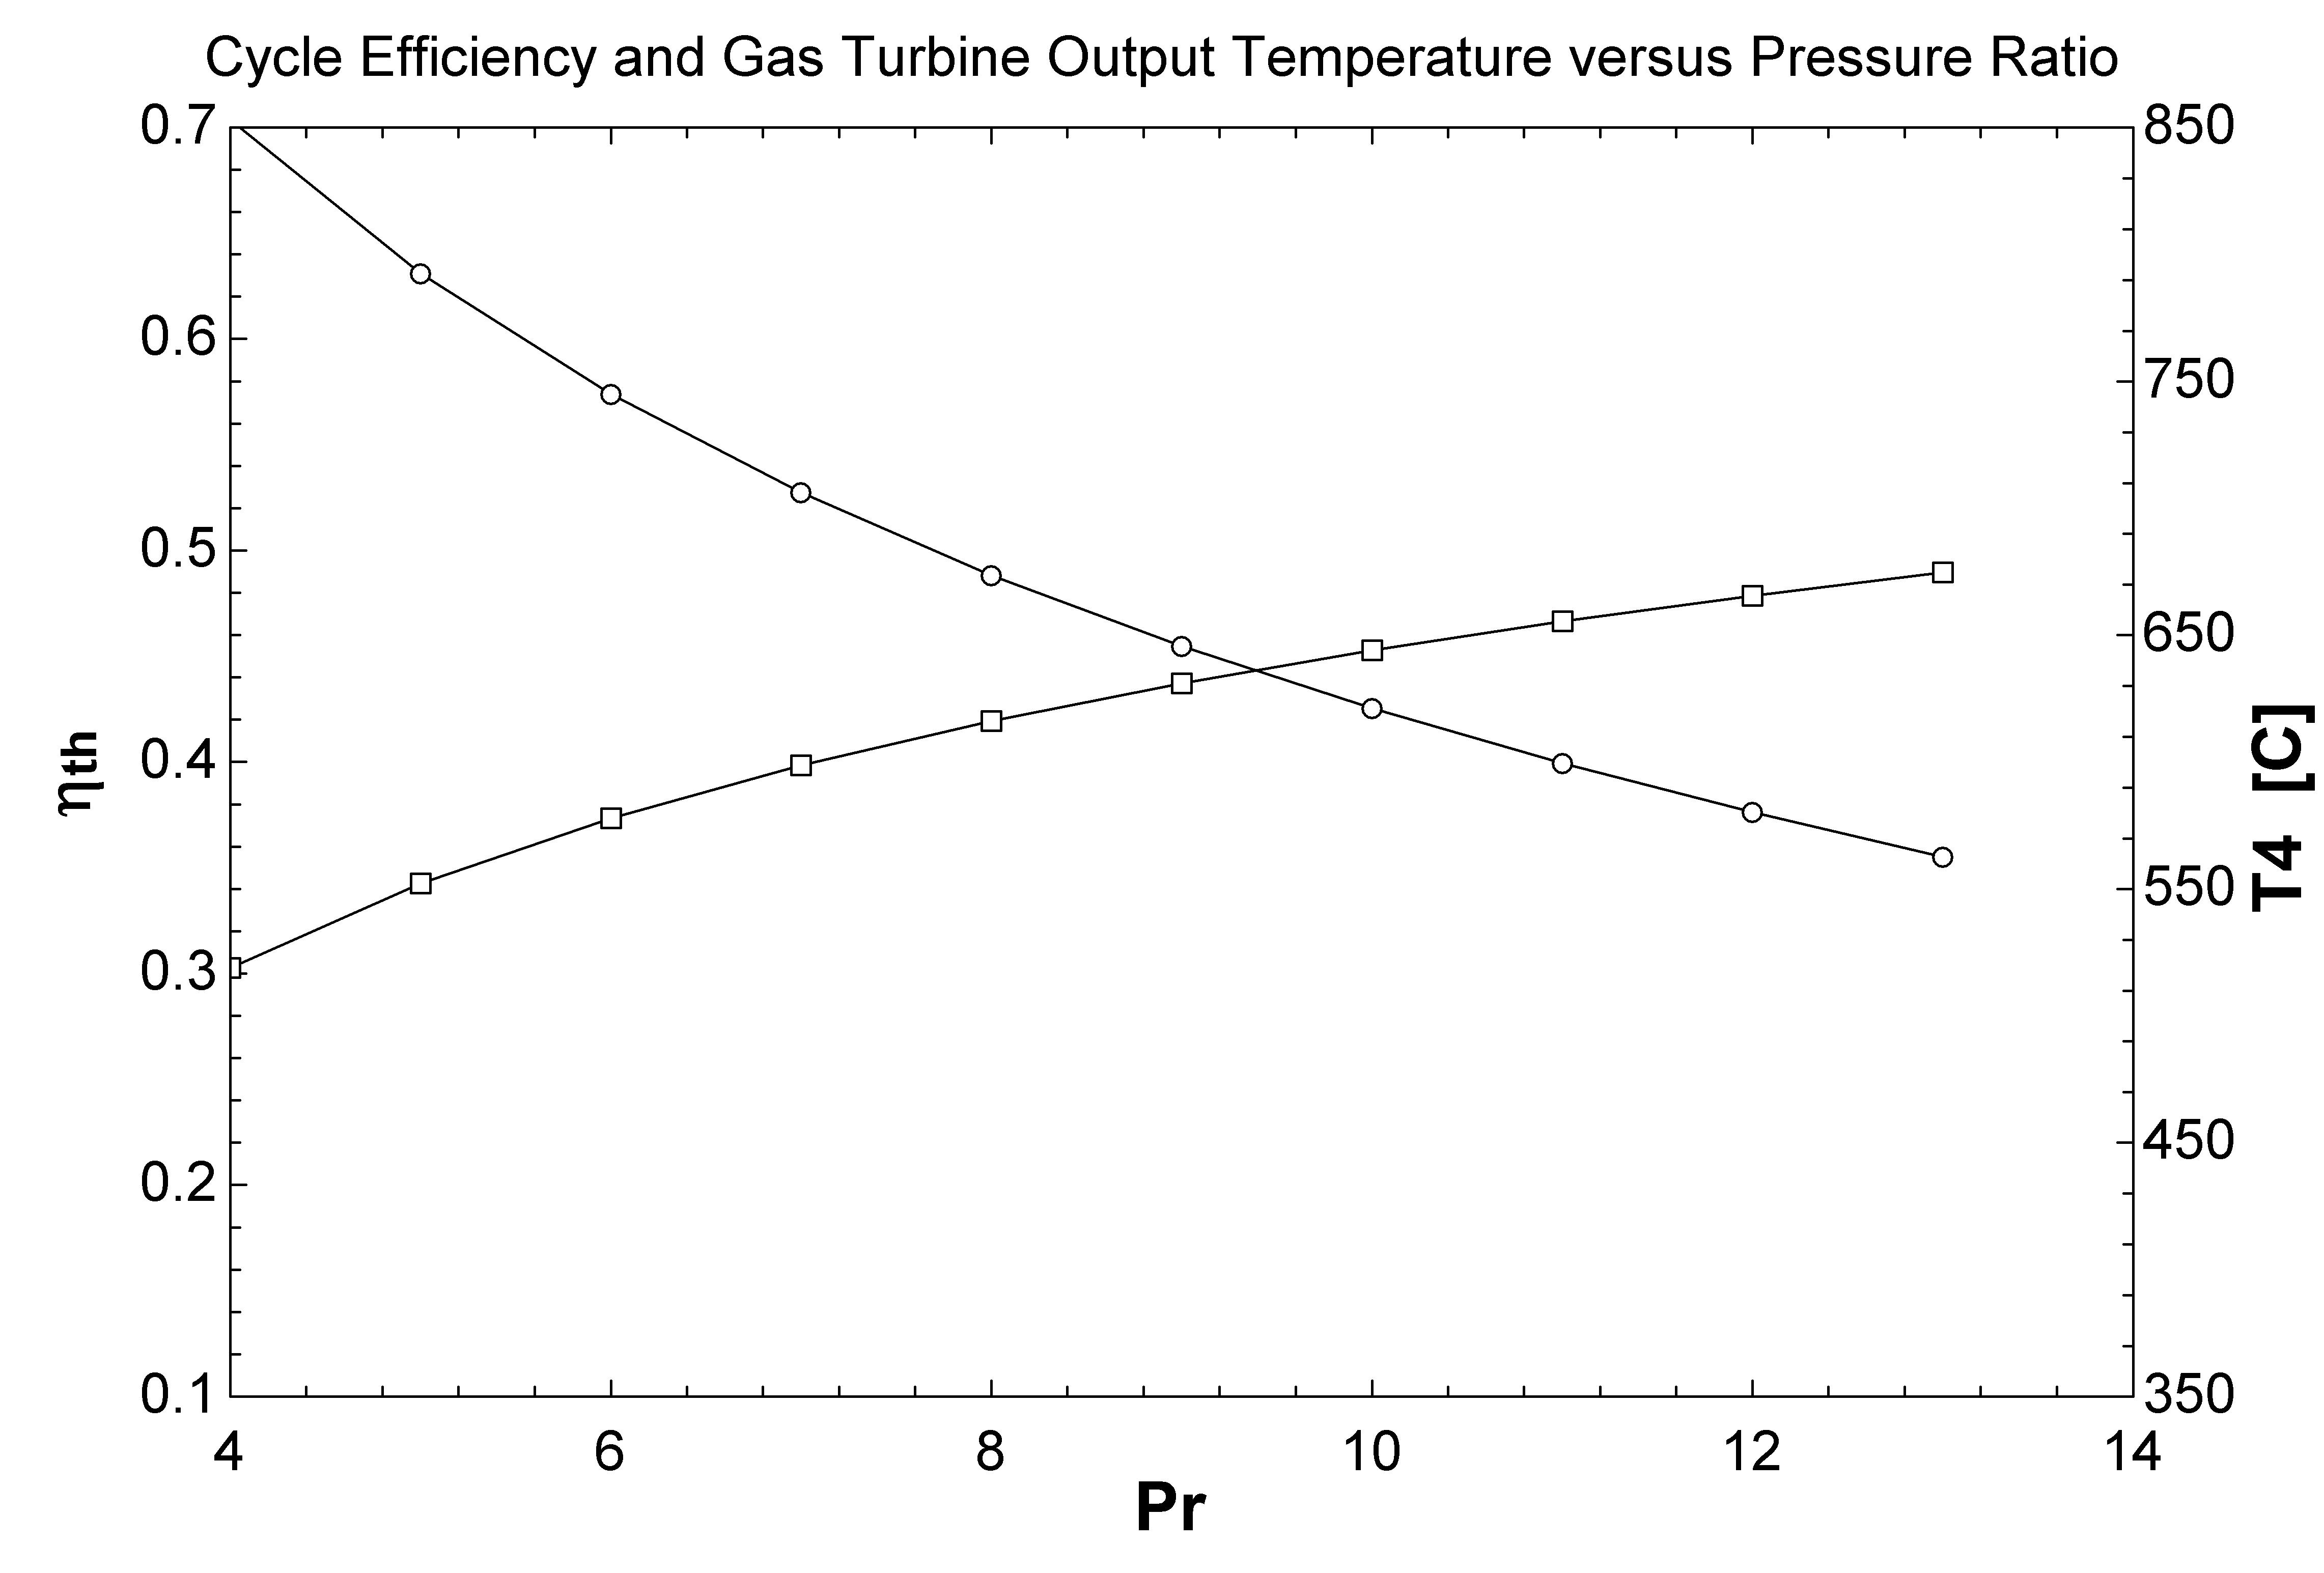
\includegraphics[width=5.0in,keepaspectratio]{megn361_ees_miniProject_JayD_P3.jpg}}
\end{document}
